\chapter{Momentum}

\begin{marginfigure}%
  \includegraphics[width=\linewidth]{momentum.jpg}
  \caption{Soul Persona released the hot single \textit{Momentum} in October of 2015.  It's mediocre R\&B synth-pop with great album art.}
  \label{fig:marginfig}
\end{marginfigure}
\textit{Confusion is the beginning of wisdom.}  \\
\noindent\textbf{-   Socrates}


\section{Force, Momentum, Impulse}

\newthought{In classical mechanics}, translational momentum is the product of the mass and velocity of an object.  Since velocity is a vector quantity, momentum is also a vector quantity.
$$\overrightarrow{p}=m\overrightarrow{v}$$

For example, a heavy spaceship moving rapidly has a large momentum.  It takes a large or prolonged force to get the spaceship up to this speed, and it takes a large or prolonged force to bring it to a stop afterwards. If the truck were less massive, or moving more slowly, then it would have less momentum.


\vspace{1cm}

The net force on an object is the time rate of change of the momentum.  This is an alternate representation of Newton's second law.

$$\overrightarrow{F}_{net}=m\overrightarrow{a}=\lim_{\Delta \rightarrow 0}\frac{\Delta \overrightarrow{p}}{\Delta t}$$
$$\left<\overrightarrow{F}_{net}\right>=\frac{\Delta\overrightarrow{p}}{\Delta t}$$

\newthought{Impulse} is the accumulated effect of a force over time.  It is also the change in momentum.  Impulse is also a vector quantity.  Graphically, impulse is the area beneath the $F_{net}(t)$ graph.
$$\overrightarrow{J}=\Delta \overrightarrow{p}=\text{Area}\left( \overrightarrow{F}_{net}(t)\right)$$



\begin{marginfigure}[-200pt]%
\pgfmathdeclarefunction{gauss}{2}{%
  \pgfmathparse{1/(#2*sqrt(2*pi))*exp(-((x-#1)^2)/(2*#2^2))}%
}

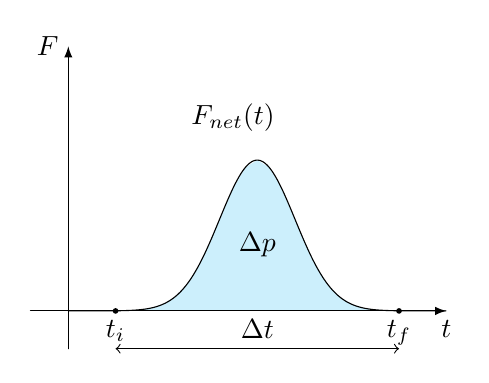
\begin{tikzpicture}
    [line cap=round,line join=round,x=2cm,y=2cm, scale=1.2, decoration={brace,amplitude=2pt}]
%main layer
%creating the ticks and xy-axis nodes
%some function
\fill[fill=cyan!20] (0.25,0) -- plot [domain=0.25:1.75] (\x,{2/(sqrt(2*pi))*exp(-((\x-1)^2)/(2*0.2^2))}) -- plot [domain=0.75: 0.25] (\x,0) -- cycle;

 \draw[smooth,samples=200,domain=0:2]
                                 plot(\x,{2/(sqrt(2*pi))*exp(-((\x-1)^2)/(2*0.2^2))});
 

    \fill[black] (0.25,0) circle (0.3mm) node [anchor=north ,scale=1] {$ t_i$};
     \fill[black] (1.75,0) circle (0.3mm) node [anchor=north ,scale=1] {$t_f$};
      %  \fill[black] (0,0.25) circle (0.3mm) node [anchor=south east,scale=1] {\scriptsize$ v(0)$};

  \draw[-latex,color=black,thin] (-0.2,0) -- (2,0) node [anchor=north ,scale=1] {$t$};
   \draw[-latex,color=black,thin] (0,-0.2) -- (0,1.4)node [anchor=east ,scale=1] {$F$};
    \draw (0.6,0.9) node [anchor=south west ,scale=1] {$F_{net}(t)$};
        \draw (1,0.35) node [anchor=center ,scale=1] {$\Delta p$};
         \draw[<->,color=black,thin] (0.25,-0.2) -- (1.75,-0.2)node [midway,anchor=south ,scale=1] {$\Delta t$};
        
 \end{tikzpicture}
  \caption{Impulse is the area under the curve in a force versus time graph.}
  \label{fig:marginfig}
\end{marginfigure}



\newpage

\begin{marginfigure}[40pt]%
  \includegraphics[width=\linewidth]{astronauts.jpg}
  \caption{Two astronauts in deep space are good examples of a system with no external forces.  The total momentum of the two astronauts is conserved unless the earth exerts an external gravitational force or George Clooney fires his thruster.   }
  \label{fig:marginfig}
\end{marginfigure}

\section{Conservation of Momentum}
\newthought{Total momentum is constant} in a closed system, one that does not exchange any matter with its surroundings and is not acted on by external forces. This fact, known as the law of conservation of momentum, is implied by Newton's laws of motion.

Start with Newton's third law.
$$\overrightarrow{F}_{12}=-\overrightarrow{F}_{21}$$
If there are no external forces then the force of particle one on particle two is the net force on particle two and the force of particle two on particle one is the net force on particle two.  
$$\overrightarrow{F}_{2net}=-\overrightarrow{F}_{1net}$$
Next we invoke Newton's second law.
$$\frac{\Delta \overrightarrow{p}_{2}}{\Delta t}=-\frac{\Delta \overrightarrow{p}_{1}}{\Delta t}$$
$$\Delta \overrightarrow{p}_{2}=-\Delta \overrightarrow{p}_{1}$$
Next substitute the definition of what $\Delta p$ is.
$$\overrightarrow{p}_{2f} -\overrightarrow{p}_{2i}=-\overrightarrow{p}_{1f} +\overrightarrow{p}_{1i}$$
Finally separate the terms with final states of the left and initial states on the right.
$$\overrightarrow{p}_{2f} +\overrightarrow{p}_{1f}=\overrightarrow{p}_{1i} +\overrightarrow{p}_{2i}$$
This delivers the conservation of momentum, namely the total momentum of the system is conserved from the initial state to the final state.
$$\overrightarrow{P}_{f}=\overrightarrow{P}_{i} $$

\subsection{External Forces}
In the case of non-zero external forces on the system the total momentum of the system is not conserved.   
$$\sum{ \overrightarrow{F}_{ext}}=M\overrightarrow{a}_{cm}=\lim_{\Delta \rightarrow 0}\frac{\Delta \overrightarrow{P}}{\Delta t}$$

\newpage

\section{Moments, Centroids and Their Time Derivatives  }

\begin{marginfigure}[0pt]%
  \includegraphics[width=\linewidth]{centroid.jpg}
  \caption{Moments analysis is a general type of statistical analysis. }
  \label{fig:marginfig}
\end{marginfigure}

\newthought{A moment is} a specific quantitative measure describing the distribution of some set of points.  Moments are used in both mechanics and statistics.  If the points represent mass, then the zeroth moment is the total mass, the first moment divided by the total mass is the center of mass, and the second moment is the rotational inertia. If the points represent probability density, then the zeroth moment is the total probability (i.e. one), the first moment is the mean, the second moment is the variance.  

A centroid is another name for the center of mass.  The time rate of change of the first moment is the total momentum.  The time rate of change of the center of mass is also called the velocity of the center of mass.  It is the total momentum divided by the total mass.

\vspace{1cm}

\begin{fullwidth}
\begin{minipage}{7.5cm}
\subsection{2 Particles}
$$M=m_1+m_2$$

$$\overrightarrow{\mathcal{M}_{I}}=m_1\overrightarrow{r}_1+m_2\overrightarrow{r}_2 $$

$$\overrightarrow{P}=\lim_{\Delta \rightarrow 0}\frac{\Delta \overrightarrow{\mathcal{M}_{I}}}{\Delta t}=m_1\overrightarrow{v}_1+m_2\overrightarrow{v}_2$$

$$\overrightarrow{r}_{cm}=\frac{\overrightarrow{\mathcal{M}_{I}}}{M}=\frac{m_1\overrightarrow{r}_1+m_2\overrightarrow{r}_2}{m_1+m_2}$$

$$\overrightarrow{v}_{cm}=\lim_{\Delta \rightarrow 0}\frac{\Delta \overrightarrow{r}_{cm}}{\Delta t}=\frac{m_1\overrightarrow{v}_1+m_2\overrightarrow{v}_2}{m_1+m_2}$$
\end{minipage}
\begin{minipage}{7.5cm}
\subsection{N Particles}

$$M=\sum^N_{n=1}m_n$$

$$\overrightarrow{\mathcal{M}_{I}}=\sum^N_{n=1}m_n\overrightarrow{r}_n$$

$$\overrightarrow{P}=\sum^N_{n=1} m_n\overrightarrow{v}_n$$


$$\overrightarrow{r}_{cm}=\frac{\overrightarrow{\mathcal{M}_{I}}}{M}$$

$$\overrightarrow{v}_{cm}=\frac{\overrightarrow{P}}{M}$$


\end{minipage}



\end{fullwidth}

\vspace{0.5cm}

\begin{figure}
  \includegraphics[width=7cm]{centroids.jpg}
  \caption{Each cluster of points in this graph is assigned a centroid.  It represents the average position of the points in each cluster. }
  \label{fig:marginfig}
\end{figure}


\newpage
\section{Collisons}

\begin{marginfigure}
  \includegraphics[width=\linewidth]{europa.jpg}
  \caption{NASA's Galileo mission revealed clay-type minerals on Jupiter's moon Europa that appear to have been delivered by an inelastic collision with an asteroid or comet.}
  \label{fig:marginfig}
\end{marginfigure}

\newthought{A collision} is an event in which two or more bodies exert forces on each other for a relatively short time. Collision implies nothing about the magnitude of the forces.


$$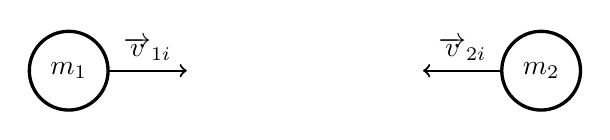
\begin{tikzpicture}[scale=1]
     	
	%\fill[black] (-7,0) circle (0.5mm);   
	%\draw[->,thick] (-7,0) -- (-6,0) node [anchor=west ,scale=1] {$F_g$}; 
	%\fill[black] (7,0) circle (0.5mm);   
%	\draw[->,thick] (7,0) -- (6,0) node [anchor=east ,scale=1] {$F_g$}; 
	 \draw[very thick] (-3,0) circle (0.5cm) node {$m_1$};
	 \draw[->,thick] (-2.5,0) -- (-1.5,0) node [anchor=south, midway ,scale=1] {$\overrightarrow{v}_{1i}$};
	  \draw[very thick] (3,0) circle (0.5cm) node {$m_2$};
	   \draw[->,thick] (2.5,0) -- (1.5,0) node [anchor=south, midway ,scale=1] {$\overrightarrow{v}_{2i}$};
	  %  \draw[thick, color=gray,->] (-4,-0.75) --   (4,-0.75) node [midway, anchor=south] {$r$};
	     
	     
	  %     \begin{scope}[shift={(-3,0)}, scale=0.75] 
	 
	   %\draw[thick](0.2,0.1) -- (0.2,-0.1);
	   % \draw[ thick,-stealth] (0.1,0) -- (1,0) node [near start,anchor=north]{\scriptsize $r$};  
	  %\end{scope}
   
	     
   \end{tikzpicture}$$
   $$\textbf{COLLISION!!!}$$
   $$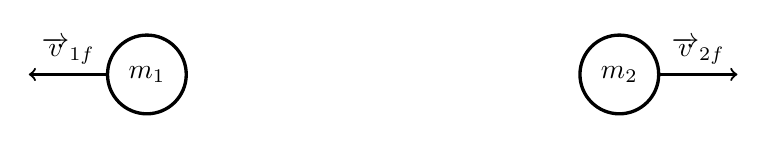
\begin{tikzpicture}[scale=1]
     	
	%\fill[black] (-7,0) circle (0.5mm);   
	%\draw[->,thick] (-7,0) -- (-6,0) node [anchor=west ,scale=1] {$F_g$}; 
	%\fill[black] (7,0) circle (0.5mm);   
%	\draw[->,thick] (7,0) -- (6,0) node [anchor=east ,scale=1] {$F_g$}; 
	 \draw[very thick] (-3,0) circle (0.5cm) node {$m_1$};
	 \draw[->,thick] (-3.5,0) -- (-4.5,0) node [anchor=south, midway ,scale=1] {$\overrightarrow{v}_{1f}$};
	  \draw[very thick] (3,0) circle (0.5cm) node {$m_2$};
	   \draw[->,thick] (3.5,0) -- (4.5,0) node [anchor=south, midway ,scale=1] {$\overrightarrow{v}_{2f}$};
	  %  \draw[thick, color=gray,->] (-4,-0.75) --   (4,-0.75) node [midway, anchor=south] {$r$};
	     
	     
	  %     \begin{scope}[shift={(-3,0)}, scale=0.75] 
	 
	   %\draw[thick](0.2,0.1) -- (0.2,-0.1);
	   % \draw[ thick,-stealth] (0.1,0) -- (1,0) node [near start,anchor=north]{\scriptsize $r$};  
	  %\end{scope}
   
	     
   \end{tikzpicture}$$

\subsection{One Dimensional Collisions}


\subsubsection{Inelastic}
\newthought{Inelastic collisions} end with the two masses sticking together therefore they end with the same final velocity.  Kinetic energy is lost in an inelastic collision.  Heat is produced.  Momentum is conserved.


$$P_f=P_i$$
$$m_1v_{1f}+m_2v_{2f}=m_1v_{1i}+m_2v_{2i}$$
The masses end with the same final velocity.
$$v_{1f}=v_{2f}=v_{f}$$
The final velocity may be calculated directly.
$$v_{f}=\frac{m_1v_{1i}+m_2v_{2i}}{m_1+m_2}$$

$$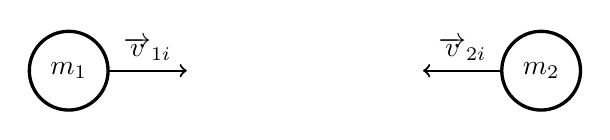
\begin{tikzpicture}[scale=1]
     	
	%\fill[black] (-7,0) circle (0.5mm);   
	%\draw[->,thick] (-7,0) -- (-6,0) node [anchor=west ,scale=1] {$F_g$}; 
	%\fill[black] (7,0) circle (0.5mm);   
%	\draw[->,thick] (7,0) -- (6,0) node [anchor=east ,scale=1] {$F_g$}; 
	 \draw[very thick] (-3,0) circle (0.5cm) node {$m_1$};
	 \draw[->,thick] (-2.5,0) -- (-1.5,0) node [anchor=south, midway ,scale=1] {$\overrightarrow{v}_{1i}$};
	  \draw[very thick] (3,0) circle (0.5cm) node {$m_2$};
	   \draw[->,thick] (2.5,0) -- (1.5,0) node [anchor=south, midway ,scale=1] {$\overrightarrow{v}_{2i}$};
	  %  \draw[thick, color=gray,->] (-4,-0.75) --   (4,-0.75) node [midway, anchor=south] {$r$};
	     
	     
	  %     \begin{scope}[shift={(-3,0)}, scale=0.75] 
	 
	   %\draw[thick](0.2,0.1) -- (0.2,-0.1);
	   % \draw[ thick,-stealth] (0.1,0) -- (1,0) node [near start,anchor=north]{\scriptsize $r$};  
	  %\end{scope}
   
	     
   \end{tikzpicture}$$
   $$\textbf{CRASH!!!}$$
   \vspace{0.5cm}
   $$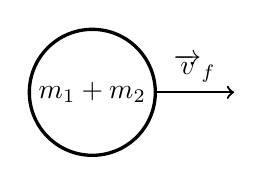
\begin{tikzpicture}[scale=1]
     	
	%\fill[black] (-7,0) circle (0.5mm);   
	%\draw[->,thick] (-7,0) -- (-6,0) node [anchor=west ,scale=1] {$F_g$}; 
	%\fill[black] (7,0) circle (0.5mm);   
%	\draw[->,thick] (7,0) -- (6,0) node [anchor=east ,scale=1] {$F_g$}; 
	% \draw[very thick] (-3,0) circle (0.5cm) node {$m_1$};
	 %\draw[->,thick] (-3.5,0) -- (-4.5,0) node [anchor=south, midway ,scale=1] {$\overrightarrow{v}_{1f}$};
	  \draw[very thick] (0,0) circle (0.8cm) node {$m_1+m_2$};
	   \draw[->,thick] (0.8,0) -- (1.8,0) node [anchor=south, midway ,scale=1] {$\overrightarrow{v}_{f}$};
	  %  \draw[thick, color=gray,->] (-4,-0.75) --   (4,-0.75) node [midway, anchor=south] {$r$};
	     
	     
	  %     \begin{scope}[shift={(-3,0)}, scale=0.75] 
	 
	   %\draw[thick](0.2,0.1) -- (0.2,-0.1);
	   % \draw[ thick,-stealth] (0.1,0) -- (1,0) node [near start,anchor=north]{\scriptsize $r$};  
	  %\end{scope}
   
	     
   \end{tikzpicture}$$
   
   \newpage
   
   \subsubsection{Elastic Collisions}
   \marginnote[0pt]{Elasticity is the ability of a body to resist a distorting influence or stress and to return to its original size and shape when the stress is removed. Solid objects will deform when forces are applied on them. If the material is elastic, the object will return to its initial shape and size when these forces are removed.

The physical reasons for elastic behavior can be quite different for different materials. In metals, the atomic lattice changes size and shape when forces are applied (energy is added to the system). When forces are removed, the lattice goes back to the original lower energy state. For rubbers and other polymers, elasticity is caused by the stretching of polymer chains when forces are applied.}


   \newthought{Elastic collisions} end with both particles bouncing off each other with no loss of kinetic energy.  Both kinetic energy and momentum are conserved during an elastic collision. 
   $$P_f=P_i$$
$$KE_f=KE_i$$
In order to find the final states of the masses the following equations must be solved simultaneously.
$$m_1v_{1f}+m_2v_{2f}=m_1v_{1i}+m_2v_{2i}$$
$$m_1v_{1f}^2+m_2v_{2f}^2=m_1v_{1i}^2+m_2v_{2i}^2$$

\begin{marginfigure}[0pt]
  \includegraphics[width=\linewidth]{nanorubber.jpg}
  \caption{Network of randomly orientated carbon nanotubes forming a rubber-like viscoelastic material that is stable at extreme temperatures}
  \label{fig:marginfig}
\end{marginfigure}

$$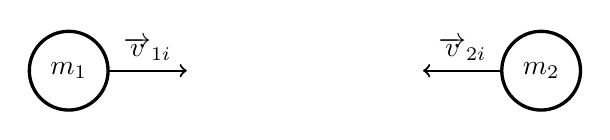
\begin{tikzpicture}[scale=1]
	 \draw[very thick] (-3,0) circle (0.5cm) node {$m_1$};
	 \draw[->,thick] (-2.5,0) -- (-1.5,0) node [anchor=south, midway ,scale=1] {$\overrightarrow{v}_{1i}$};
	  \draw[very thick] (3,0) circle (0.5cm) node {$m_2$};
	   \draw[->,thick] (2.5,0) -- (1.5,0) node [anchor=south, midway ,scale=1] {$\overrightarrow{v}_{2i}$};
   \end{tikzpicture}$$
   $$\textbf{BOING!!!}$$
   $$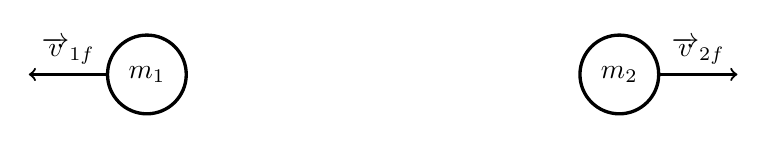
\begin{tikzpicture}[scale=1]
	 \draw[very thick] (-3,0) circle (0.5cm) node {$m_1$};
	 \draw[->,thick] (-3.5,0) -- (-4.5,0) node [anchor=south, midway ,scale=1] {$\overrightarrow{v}_{1f}$};
	  \draw[very thick] (3,0) circle (0.5cm) node {$m_2$};
	   \draw[->,thick] (3.5,0) -- (4.5,0) node [anchor=south, midway ,scale=1] {$\overrightarrow{v}_{2f}$};
   \end{tikzpicture}$$


\section{Center of Mass Coordinates}
\newthought{A center of mass coordinate system} shifts the frame of reference to that of the velocity of the center of mass.  The velocities of the masses are calculated relative to the velocity of the center of mass.  An underscore is used to notate velocities which are in the center of mass coordinate system.  

First the velocity of the center of mass is calculated.
$$\overrightarrow{v}_{cm}=\frac{m_1\overrightarrow{v}_1+m_2\overrightarrow{v}_2}{m_1+m_2}$$
Once the velocity of the center of mass is determined the velocities of each mass relative to the center of mass may be calculated.
$$\overrightarrow{\underbar{v}}=\overrightarrow{v}-\overrightarrow{v}_{cm}$$
In a center of mass coordinate system the total momentum of the system is zero.
$$\overrightarrow{\underbar{p}}=m\overrightarrow{\underbar{v}}=m\overrightarrow{v}-m\overrightarrow{v}_{cm}$$
$$\overrightarrow{\underbar{P}}=0$$


\newpage
\section{1-D Collisions}
\marginnote[0pt]{Trucking, tracking, dollying and crabbing are all terms for the technique of putting a camera on a platform (dolly) that slides along a track.  In trucking the camera moves side to side, perpendicular its optical axis.}
\vspace{1cm}
\subsection{Inelastic}
For an inelastic collision the final velocity of the masses is the velocity of the center of mass.
$$\underbar{P}_f=\underbar{P}_i=0$$
$$\underbar{v}_{1f}=\underbar{v}_{2f}=0$$
$$v_{1f}=v_{2f}=v_{cm}$$

\begin{marginfigure}
  \includegraphics[width=\linewidth]{track.jpg}
  \caption{Center of mass coordinates are tracking shots of which make the total momentum of the system zero. }
  \label{fig:marginfig}
\end{marginfigure}

$$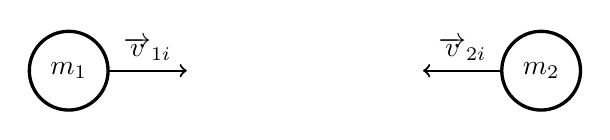
\begin{tikzpicture}[scale=1]
	 \draw[very thick] (-3,0) circle (0.5cm) node {$m_1$};
	 \draw[->,thick] (-2.5,0) -- (-1.5,0) node [anchor=south, midway ,scale=1] {$\overrightarrow{v}_{1i}$};
	  \draw[very thick] (3,0) circle (0.5cm) node {$m_2$};
	   \draw[->,thick] (2.5,0) -- (1.5,0) node [anchor=south, midway ,scale=1] {$\overrightarrow{v}_{2i}$};
   \end{tikzpicture}$$
   
   $$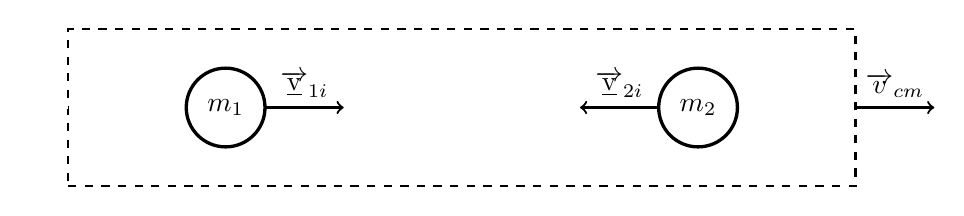
\begin{tikzpicture}[scale=1]
   \draw[dashed,thick] (-5,-1) -- (5,-1) -- (5,1) -- (-5,1) -- (-5,-1);
	 \draw[very thick] (-3,0) circle (0.5cm) node {$m_1$};
	  \draw[->,thick] (5,0) -- (6,0) node [anchor=south, midway ,scale=1] {$\overrightarrow{v}_{cm}$};
	  \draw[->,thick,color=white] (-5,0) -- (-5.5,0);
	 \draw[->,thick] (-2.5,0) -- (-1.5,0) node [anchor=south, midway ,scale=1] {$\overrightarrow{\underbar{v}}_{1i}$};
	  \draw[very thick] (3,0) circle (0.5cm) node {$m_2$};
	   \draw[->,thick] (2.5,0) -- (1.5,0) node [anchor=south, midway ,scale=1] {$\overrightarrow{\underbar{v}}_{2i}$};
   \end{tikzpicture}$$
   
   $$\textbf{CRASH!!!}$$
   
   $$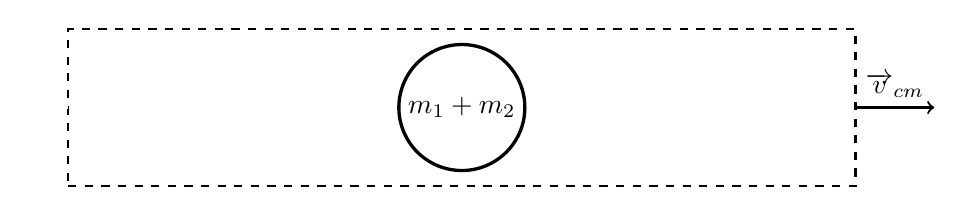
\begin{tikzpicture}[scale=1]
    \draw[dashed,thick] (-5,-1) -- (5,-1) -- (5,1) -- (-5,1) -- (-5,-1);
      \draw[->,thick] (5,0) -- (6,0) node [anchor=south, midway ,scale=1] {$\overrightarrow{v}_{cm}$};
      \draw[->,thick,color=white] (-5,0) -- (-5.5,0);
	 \draw[very thick] (0,0) circle (0.8cm) node {$m_1+m_2$};
   \end{tikzpicture}$$
   
 $$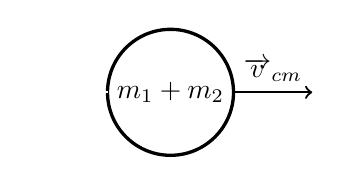
\begin{tikzpicture}[scale=1]
	  \draw[very thick] (0,0) circle (0.8cm) node {$m_1+m_2$};
	   \draw[->,thick] (0.8,0) -- (1.8,0) node [anchor=south, midway ,scale=1] {$\overrightarrow{v}_{cm}$};	
	    \draw[->,thick,color=white] (-0.8,0) -- (-1.8,0) node [anchor=south, midway ,scale=1] {$\overrightarrow{v}_{cm}$};	     
   \end{tikzpicture}$$

\newpage

\subsection{Elastic} 

\begin{marginfigure}
  \includegraphics[width=\linewidth]{running.jpg}
  \caption{This Pokemon tracking shot is from a viewpoint moving at the velocity if the center of mass }
  \label{fig:marginfig}
\end{marginfigure}

Here is where one gets their money's worth for using center of mass coordinates.  Begin with conservation of momentum and kinetic energy.
$$\underbar{P}_f=\underbar{P}_i=0$$
$$\underbar{KE}_f=\underbar{KE}_i$$
Calculate the center of mass velocity.
$$\overrightarrow{v}_{cm}=\frac{m_1\overrightarrow{v}_1+m_2\overrightarrow{v}_2}{m_1+m_2}$$
Next determine the velocity of each mass in the center of mass velocity frame.
$$\underbar{v}_{1i}={v}_{1i}-v_{cm} \hspace{1cm} \underbar{v}_{2i}={v}_{2i}-v_{cm}$$
In the center of mass coordinate system the masses simply switch direction after collision.  This is the only way to maintain zero momentum and conserve kinetic energy.
$$\underbar{v}_{1f}=-\underbar{v}_{1i} \hspace{1cm} \underbar{v}_{2f}=-\underbar{v}_{2i}$$
Finally convert back to the original coordinate system.
$$v_{1f}=2v_{cm}-v_{1i} \hspace{1cm} v_{2f}=2v_{cm}-v_{2i}$$



$$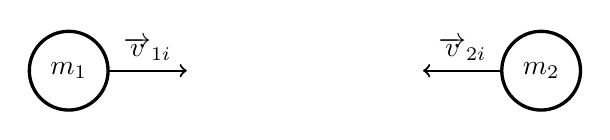
\begin{tikzpicture}[scale=1]
	 \draw[very thick] (-3,0) circle (0.5cm) node {$m_1$};
	 \draw[->,thick] (-2.5,0) -- (-1.5,0) node [anchor=south, midway ,scale=1] {$\overrightarrow{v}_{1i}$};
	  \draw[very thick] (3,0) circle (0.5cm) node {$m_2$};
	   \draw[->,thick] (2.5,0) -- (1.5,0) node [anchor=south, midway ,scale=1] {$\overrightarrow{v}_{2i}$};
   \end{tikzpicture}$$
   
   $$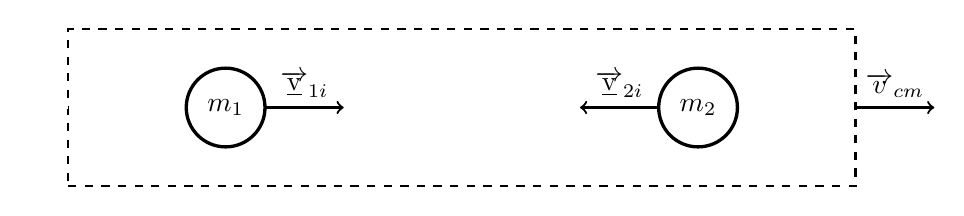
\begin{tikzpicture}[scale=1]
   \draw[dashed,thick] (-5,-1) -- (5,-1) -- (5,1) -- (-5,1) -- (-5,-1);
	 \draw[very thick] (-3,0) circle (0.5cm) node {$m_1$};
	  \draw[->,thick] (5,0) -- (6,0) node [anchor=south, midway ,scale=1] {$\overrightarrow{v}_{cm}$};
	  \draw[->,thick,color=white] (-5,0) -- (-5.5,0);
	 \draw[->,thick] (-2.5,0) -- (-1.5,0) node [anchor=south, midway ,scale=1] {$\overrightarrow{\underbar{v}}_{1i}$};
	  \draw[very thick] (3,0) circle (0.5cm) node {$m_2$};
	   \draw[->,thick] (2.5,0) -- (1.5,0) node [anchor=south, midway ,scale=1] {$\overrightarrow{\underbar{v}}_{2i}$};
   \end{tikzpicture}$$
   
   $$\textbf{BOING!!!}$$
   
   $$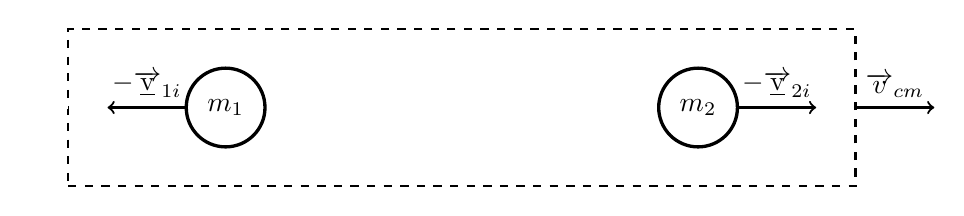
\begin{tikzpicture}[scale=1]
    \draw[dashed,thick] (-5,-1) -- (5,-1) -- (5,1) -- (-5,1) -- (-5,-1);
      \draw[->,thick] (5,0) -- (6,0) node [anchor=south, midway ,scale=1] {$\overrightarrow{v}_{cm}$};
      \draw[->,thick,color=white] (-5,0) -- (-5.5,0);
	 \draw[very thick] (-3,0) circle (0.5cm) node {$m_1$};
	 \draw[->,thick] (-3.5,0) -- (-4.5,0) node [anchor=south, midway ,scale=1] {$-\overrightarrow{\underbar{v}}_{1i}$};
	  \draw[very thick] (3,0) circle (0.5cm) node {$m_2$};
	   \draw[->,thick] (3.5,0) -- (4.5,0) node [anchor=south, midway ,scale=1] {$-\overrightarrow{\underbar{v}}_{2i}$};

   \end{tikzpicture}$$
   
    $$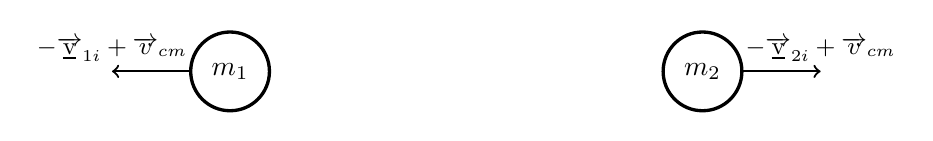
\begin{tikzpicture}[scale=1]
    %\draw[dashed,thick] (-5,-1) -- (5,-1) -- (5,1) -- (-5,1) -- (-5,-1);
     % \draw[->,thick] (5,0) -- (6,0) node [anchor=south, midway ,scale=1] {$\overrightarrow{v}_{cm}$};
      %\draw[->,thick,color=white] (-5,0) -- (-5.5,0);
	 \draw[very thick] (-3,0) circle (0.5cm) node {$m_1$};
	 \draw[->,thick] (-3.5,0) -- (-4.5,0) node [anchor=south ,scale=1] {\small$-\overrightarrow{\underbar{v}}_{1i}+\overrightarrow{v}_{cm}$};
	  \draw[very thick] (3,0) circle (0.5cm) node {$m_2$};
	   \draw[->,thick] (3.5,0) -- (4.5,0) node [anchor=south ,scale=1] {\small$-\overrightarrow{\underbar{v}}_{2i}+\overrightarrow{v}_{cm}$};

   \end{tikzpicture}$$

